% lintrans - The linear transformation visualizer
% Copyright (C) 2021-2022 D. Dyson (DoctorDalek1963)

% This program is licensed under GNU GPLv3, available here:
% <https://www.gnu.org/licenses/gpl-3.0.html>

\documentclass[../development.tex]{subfiles}

\begin{document}

It's not universal, but the word \enquote{eigenstuffs} is common enough in mathematics that I'm comfortable using it here to mean eigenvalues, eigenvectors, and eigenlines, where an eigenline is the span of an eigenvector.

\subsubsection{Drawing eigenvectors\label{development:implementing-eigenstuffs:drawing-eigenvectors}}

An eigenvector $\mathbf{v}$ of a matrix $\mathbf{M}$ is a vector that satisfies the equation $\mathbf{Mv} = \lambda\mathbf{v}$ for some scalar $\lambda$. Thankfully, I don't have to worry about actually computing $\mathbf{v}$ or $\lambda$, since NumPy has the \pyinline{numpy.linalg.eig()} function\cite{numpy-docs-linalg-eig}.

This function takes a square matrix and returns an array of eigenvalues ($\lambda$), and a matrix of their associated eigenvectors ($\mathbf{v}$). Some matrices don't have any real eigenvalues, but all $2 \times 2$ matrices will have 2 (possibly complex) eigenvalues, as a direct consequence of the Fundamental Theorem of Algebra\footnote{%
	$\mathbf{Mv} = \lambda\mathbf{v} \implies \mathbf{Mv} = \lambda\mathbf{I}\mathbf{v} \implies (\mathbf{M} - \lambda\mathbf{I})\mathbf{v} = \mathbf{0} \implies \det(\mathbf{M} - \lambda\mathbf{I}) = 0\text{ (since we only want non-zero vectors)}\\%
\implies \begin{vmatrix}a - \lambda & b\\ c & d - \lambda\end{vmatrix} = 0 \implies (a - \lambda)(d - \lambda) - bc = 0 \implies \lambda^2 - (a + d)\lambda + (ad - bc) = 0 \\%
\implies \lambda$ has 2 solutions in $\mathbb{C}$ by the Fundamental Theorem of Algebra\cite{the-fundamental-theorem-of-algebra}%
}. We don't want to try to render an eigenvector if its eigenvalue is complex, so we have to check and only render the real ones. Python doesn't distinguish really between \pyinline{float} and \pyinline{complex} types, so we can just check the \pyinline{.imag} property no matter what. If it's 0, then we keep the eigenvalue. NumPy normalizes the eigenvectors to have a length of 1, but I'd much prefer them to have a length equal to their associated eigenvalue. To do that, we can just multiply the eigenvectors by their eigenvalues.

We then just draw a vector, consisting of a line and an arrowhead, from the origin to the extended eigenvector.

%: b8614334de5cba4b1a6d92508b08fa8bd2fe77c0
%: src/lintrans/gui/plots/classes.py:163,450-465

%: b8614334de5cba4b1a6d92508b08fa8bd2fe77c0
%: src/lintrans/gui/plots/widgets.py:58

At this point in development, I didn't particularly care about the colours of various elements. It was more important to get things working first, so I ended up choosing \textcolor[RGB]{255, 249, 0}{this horrible yellow} for the eigenvectors. It's clearly an awful choice for text, and it's not very good for the eigenvectors either, since it makes them hard to see against the white background. I wasn't really considering the usability features discussed in \S\ref{design:usability-features}, but since I was the only user, and changing a few colours later on wouldn't be much work, I wasn't worried about it.

\begin{figure}[H]
	\centering
	\includegraphics[width=0.8\linewidth]{development/b8614334de5cba4b1a6d92508b08fa8bd2fe77c0/gui.png}
	\caption{The eigenvectors being displayed for an arbitrary matrix}
	\label{fig:development:b8614334de5cba4b1a6d92508b08fa8bd2fe77c0:gui.png}
\end{figure}

\subsubsection{Adding display settings for eigenvectors\label{development:implementing-eigenstuffs:adding-display-settings-for-eigenvectors}}

Once I'd got the eigenvectors working and being drawn, I wanted to be able to turn them on and off from the display settings. This was a simple case of just adding it to the \pyinline{DisplaySettings} dataclass, adding the checkbox to the dialog, and only drawing the eigenvectors if this display setting is true.

%: 3ebb5997a7a887e751b5f4f717aa5161ed013e62
%: src/lintrans/gui/settings.py:41-42

%: 3ebb5997a7a887e751b5f4f717aa5161ed013e62
%: src/lintrans/gui/dialogs/settings.py:123-126

%: 3ebb5997a7a887e751b5f4f717aa5161ed013e62
%: src/lintrans/gui/plots/widgets.py:58-59

\subsubsection{Refactoring drawing vectors\label{development:implementing-eigenstuffs:refactoring-drawing-vectors}}

Since I've now got several drawing methods that involve drawing vectors, I thought I should factor out this functionality into a separate utility method which I could call from all these places.

%: 754eba0318a682b068a8a5d5ca451decbaa204ce
%: src/lintrans/gui/plots/classes.py:388-406,454-466

When I was testing this refactor, I realised that the \pyinline{draw_transformed_grid()} method originally drew the bodies of the basis vectors and the caller had to draw the arrowheads separately. This is silly and was never planned that way; it was an unfortunate consequence of implementing the lines and arrowheads at different times. But now after this refactor, the caller has to call \pyinline{draw_basis_vectors()} to draw the whole basis vectors. So I had to add this call to \pyinline{VisualizeTransformationWidget.paintEvent()} and \pyinline{DefineVisuallyWidget.paintEvent()} in \texttt{src/lintrans/gui/plots/widgets.py} and remove the calls to \pyinline{draw_vector_arrowheads()}.

\subsubsection{Adding eigenlines\label{development:implementing-eigenstuffs:adding-eigenlines}}

Drawing some eigenvectors that point in a general direction is fine, but drawing the whole span of the vector would be much more useful. These spans are called eigenlines, and are just lines in the direction of the vector. To implement these, I knew I would have to get the eigenvalues and eigenvectors, zip them, and iterate over them like I did in \S\ref{development:implementing-eigenstuffs:drawing-eigenvectors}. To make this simpler, I decided to factor out this zipping into a separate \pyinline{self.eigs} property\footnote{A \pyinline{@property} in Python is a value on a class which is dynamically evaluated only when it's needed. It functions just like a method with no arguments, but has more concise syntax for the caller.}.

%: e1606f1e45ba93102dddb74b45ab22649a63fa53
%: src/lintrans/gui/plots/classes.py:187-194,465-474

I could then create a new method to find the gradient of the vector line and draw an orthogonal or oblique line respectively. Like before, we only want to render the eigenlines for real-valued eigenvectors, so we have to check their imaginary part.

%: 8d4d41fc4780cc037be39a0e574158e6cd34e997
%: src/lintrans/gui/plots/classes.py:476-498

I then just had to put these new eigenlines behind a display setting.

%: 12cfabde606ebd3d48b2c3efaad0412f6100c3c5
%: src/lintrans/gui/settings.py:44-45

%: 12cfabde606ebd3d48b2c3efaad0412f6100c3c5
%: src/lintrans/gui/dialogs/settings.py:128-131

%: 12cfabde606ebd3d48b2c3efaad0412f6100c3c5
%: src/lintrans/gui/plots/widgets.py:58-59

\begin{figure}[H]
	\centering
	\includegraphics[width=0.8\linewidth]{development/12cfabde606ebd3d48b2c3efaad0412f6100c3c5/gui.png}
	\caption{The eigenvectors being displayed for a similar matrix as in Figure~\ref{fig:development:b8614334de5cba4b1a6d92508b08fa8bd2fe77c0:gui.png}}
	\label{fig:development:12cfabde606ebd3d48b2c3efaad0412f6100c3c5:gui.png}
\end{figure}

\subsubsection{A tiny UI change\label{development:implementing-eigenstuffs:a-tiny-ui-change}}

\begin{figure}[H]
	\begin{minipage}{0.35\linewidth}
		\centering
		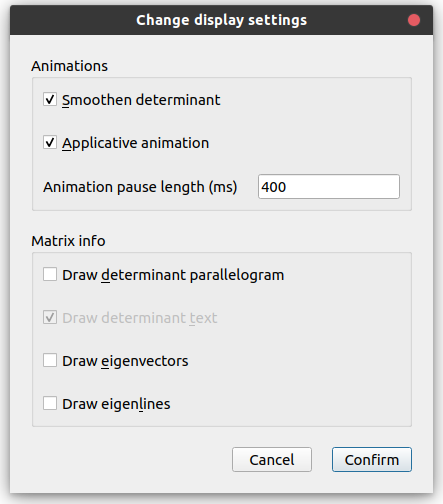
\includegraphics[width=\linewidth]{development/90425137edd4596219ab564ccbeccd65b5754008/display_settings.png}
		\caption{The display settings}
		\label{fig:development:90425137edd4596219ab564ccbeccd65b5754008:display_settings.png}
	\end{minipage}\hfill
	\begin{minipage}{0.6\linewidth}\setspacing
		This bit isn't really related to eigenvectors, but it's a tiny change and it doesn't really have a good place anywhere else. I really liked the groupboxes used in the display settings (left) and I'd quite like to enclose the matrix definition buttons in their own groupbox to separate them from the rest of the UI and better associate them with the label above them. This was a trivial addition.
	\end{minipage}
	\vspace{-1em}
\end{figure}

%: 90425137edd4596219ab564ccbeccd65b5754008
%: src/lintrans/gui/main_window.py:173-180,226

\begin{figure}[H]
	\hspace{0.08\linewidth}
	\begin{minipage}{0.35\linewidth}
		\centering
		\includegraphics[width=\linewidth]{development/12cfabde606ebd3d48b2c3efaad0412f6100c3c5/definition_buttons.png}
		\caption{The old matrix definition buttons}
		\label{fig:development:12cfabde606ebd3d48b2c3efaad0412f6100c3c5:definition_buttons.png}
	\end{minipage}\hfill
	\begin{minipage}{0.35\linewidth}
		\centering
		\includegraphics[width=\linewidth]{development/90425137edd4596219ab564ccbeccd65b5754008/definition_buttons.png}
		\caption{The new matrix definition buttons}
		\label{fig:development:90425137edd4596219ab564ccbeccd65b5754008:definition_buttons.png}
	\end{minipage}
	\hspace{0.08\linewidth}
\end{figure}

\end{document}
